\documentclass[twocolumn]{aastex631}
\usepackage{amsmath}
\usepackage{amssymb}
\usepackage{booktabs}

\shorttitle{Partition of Cosmological Tensions}
\shortauthors{Martin}

\begin{document}

\title{The Partition of Cosmological Tensions: \\
       Frame Artifacts, Local Structure, and Physical Residuals}

\author[0009-0006-5944-1742]{Eric D. Martin}
\affiliation{All Your Baseline LLC}
\email{eric@aybllc.com}

\begin{abstract}
We apply $\xi$-normalized coordinates ($\xi \equiv d_c / d_H$, where $d_H = c/H_0$)
to partition ten cosmological tensions into three distinct classes:
(1) coordinate-frame artifacts arising from $H_0$-dependent measurement comparisons,
(2) local-structure effects including the KBC void and bulk flows, and
(3) genuine physical residuals requiring new cosmological physics.
Across the full tension landscape --- Hubble constant, matter clustering ($S_8$),
baryon acoustic oscillations, lensing amplitude ($A_L$), age, and Lyman-$\alpha$
forest --- we find that $\sim$93\% of the $H_0$ tension is a frame artifact,
64\% of the local-expansion anomaly is explained by the KBC void and bulk flow,
and the strong-lensing H0LiCOW tension is fully accounted for by the
mass-sheet degeneracy.
The physical residuals converge on two signals: a matter density deficit
($\Omega_m \approx 0.295$, confirmed by DESI DR1) and an evolving dark energy
equation of state ($w_0 = -0.634$, $w_a = -1.388$, $\Delta\chi^2 = 4.74$).
A multi-probe convergence test demonstrates that the DESI low-$z$ BAO
$w_0 w_a$ fit extrapolates to the Ly-$\alpha$ BAO at $z=2.33$ within $0.94\sigma$,
suggesting a coherent dark energy evolution signal across $z = 0.3$--$2.3$.
These results are pre-registered ahead of the Euclid DR1 release
(October 2026), which provides the decisive test.
\end{abstract}

\keywords{cosmological parameters --- dark energy --- large-scale structure ---
          Hubble constant --- Lyman-alpha forest}

%% ─── 1. INTRODUCTION ────────────────────────────────────────────────────────

\section{Introduction}

The past decade has witnessed the emergence of several statistically significant
discrepancies between cosmological parameter values inferred from early-universe
observations (principally the cosmic microwave background; CMB) and late-universe
probes (Cepheid distance ladders, weak gravitational lensing, baryon acoustic
oscillations, and quasar spectra).
The most prominent of these is the ``Hubble tension'': a $4$--$5\sigma$ discrepancy
between the locally measured expansion rate ($H_0 = 73.04 \pm 1.04$ km s$^{-1}$ Mpc$^{-1}$;
\citealt{Riess2022}) and the CMB-inferred value ($H_0 = 67.4 \pm 0.5$ km s$^{-1}$ Mpc$^{-1}$;
\citealt{Planck2020}).

The dominant response to these tensions has been to propose modifications to the
standard $\Lambda$CDM model --- early dark energy, interacting dark matter,
modified gravity --- or to search for unidentified systematic errors in one or more
datasets \citep{DiValentino2021}.
A complementary possibility, which we investigate here, is that a significant
fraction of the apparent tension is a \emph{coordinate-frame artifact}: a consequence
of comparing measurements that implicitly assume different values of $H_0$ in their
distance definitions.

In \citet{Martin2026a} (hereafter Paper~I), we demonstrated that the redshift-scaled
comoving distance $\xi \equiv d_c / d_H = d_c H_0 / c$ provides a frame-independent
coordinate in which $H_0$-dependent systematics cancel to first order.
Applied to the SH0ES Cepheid calibrator sample, $\xi$-normalization reduces the
apparent $H_0$ discrepancy by $\sim$93\%, recovering a physical residual of
$\sim$7\% attributable to a matter density deficit rather than an expansion rate
anomaly.

Here we extend this framework to the full landscape of cosmological tensions,
providing a unified partition into frame artifacts, local-structure effects, and
physical residuals.
Our goal is not to resolve the tensions by fiat, but to identify precisely
\emph{where} new physics is required and where it is not.

We address a potential confusion at the outset.
The $H_0$ tension is often described as a disagreement about the \emph{value}
of $H_0$, not a distance comparison --- and $H_0$ is a physical observable,
not a coordinate choice.
This is correct, and $\xi$-normalization does not dispute it.
What we claim is narrower: that the \emph{significance} of the discrepancy ---
the $5\sigma$ number --- is inflated because SH0ES distances at higher
redshift are kinematically derived under an assumed cosmology, while Planck
distances are derived under a different assumed cosmology, and the two pipelines
are compared without a common frame.
The inflation is not in $H_0$ itself but in the apparent tension statistic.
$\xi$-normalization reveals what fraction of that statistic vanishes when both
pipelines are expressed in the same frame.
The residual $\sim$7\% is the physically meaningful signal --- and that signal
points to $\Omega_m$, not to an anomalous expansion rate.

%% ─── 2. METHODS ─────────────────────────────────────────────────────────────

\section{Methods}

\subsection{The $\xi$ Normalization}

The $\xi$-coordinate is defined as
\begin{equation}
  \xi(z) \equiv \frac{d_c(z)}{d_H} = \frac{H_0}{c} \int_0^z \frac{dz'}{E(z')},
  \label{eq:xi}
\end{equation}
where $E(z) = H(z)/H_0$ is the dimensionless Hubble parameter.
For a flat $w_0 w_a$ cosmology \citep{ChevallierPolarski2001,Linder2003},
\begin{equation}
  E(z) = \left[ \Omega_m (1+z)^3 + (1-\Omega_m)(1+z)^{3(1+w_0+w_a)}
         e^{-3w_a z/(1+z)} \right]^{1/2}.
\end{equation}
Because $\xi$ is dimensionless and $H_0$-independent, comparisons of $\xi$ values
between datasets with different assumed $H_0$ do not introduce frame-mixing artifacts.
The $H_0$-dependence is isolated in the overall scale $d_H = c/H_0$, which cancels
when residuals are expressed as $\Delta\xi / \xi$.
The spatial index $\xi$ is equivalently the normalized radial coordinate
$s_1 = r/R_H(a)$, where $R_H(a) = c/H(a)$ is the cosmological horizon radius
at scale factor $a$ derived from the Friedmann equations.
This identifies $\xi$ as the first component of the Universal Horizon Address
(UHA) spatial tuple \citep{Martin2026a}, making it a geometrical invariant
rather than a fitted parameter.

\subsection{Frame-Artifact Decomposition}

For each tension, we compute:
(1) the raw tension in conventional coordinates (km s$^{-1}$ Mpc$^{-1}$ or
dimensionless parameter ratios);
(2) the tension after $\xi$-normalization with a frame-independent anchor
$H_{0,\mathrm{ref}} = 70.0$ km s$^{-1}$ Mpc$^{-1}$ (chosen midway between
the SH0ES and Planck values; the frame-artifact fraction $f_{\rm frame}$
is insensitive to this choice at the $< 0.5\%$ level);
and (3) the physical residual, defined as the tension that persists after both
$\xi$-normalization and (where applicable) corrections for local structure.

The frame-artifact fraction is estimated as
\begin{equation}
  f_{\rm frame} = 1 - \frac{|\Delta_{\xi}|}{|\Delta_{\rm raw}|},
\end{equation}
where $\Delta_{\rm raw}$ is the raw parameter discrepancy and $\Delta_{\xi}$ is
the discrepancy after $\xi$-normalization.

\subsection{Data}

We use the following published datasets:
\begin{itemize}
  \item DESI DR1 BAO: $D_M/r_s$ and $D_H/r_s$ at 7 redshift bins,
        $z = 0.295$--$2.33$ \citep{DESI2024DR1}
  \item SH0ES Cepheid calibrators (77 hosts) from Pantheon+SH0ES \citep{Riess2022}
  \item Planck 2020 CMB: $H_0$, $\Omega_m$, $\sigma_8$ \citep{Planck2020}
  \item KiDS-1000, DES-Y3, HSC-Y3 $S_8$ measurements \citep{Asgari2021,Amon2022,Dalal2023}
  \item H0LiCOW 6-lens, TDCOSMO 7-lens, TDCOSMO+SLACS \citep{Wong2020,Millon2020,Birrer2021}
  \item eBOSS Ly-$\alpha$ BAO at $z=2.33$ \citep{duMasdesBourboux2020}
  \item KBC void density contrast and bulk flow \citep{Keenan2013,Kenworthy2019,Watkins2023}
\end{itemize}
All analyses use published summary statistics; no raw catalogs are required.
Scripts are archived at \url{https://zenodo.org/records/19230366} and the
companion repository \url{https://github.com/abba-01/uha}.

%% ─── 3. RESULTS ─────────────────────────────────────────────────────────────

\section{Results}

\subsection{The Tension Partition Table}

Table~\ref{tab:tensions} summarizes our partition of ten cosmological tensions.
The key distinction is between \emph{frame artifacts} (tensions that arise from
comparing measurements in incompatible $H_0$-dependent coordinate systems),
\emph{local-structure effects} (genuine astrophysical systematics in the nearby
universe), and \emph{physical residuals} (tensions that persist after both
corrections and require modifications to the standard cosmological model).

\begin{table*}
\centering
\caption{Partition of Cosmological Tensions via $\xi$-Normalization}
\label{tab:tensions}
\begin{tabular}{llccll}
\toprule
Tension & Probes & Frame & Local & Physical & Residual \\
        &        & artifact & structure & residual & significance \\
\midrule
$H_0$ (Cepheid) & SH0ES vs.\ Planck & $\sim$93\% & 64.5\%$^\ddagger$ & $\Omega_m$ deficit & $1.51\sigma$ \\
$H_0$ (JWST)    & JWST vs.\ Planck  & $\sim$93\% & 64.5\%$^\ddagger$ & $\Omega_m$ deficit & $1.51\sigma$ \\
BAO / $\Omega_m$ & DESI DR1         & 0\% & --- & $\Omega_m = 0.295\pm0.010$ & $2.2\sigma$ \\
$S_8$ / $\sigma_8$ & KiDS, DES, HSC & $\sim$3\%$^\S$ & --- & matter deficit & $2.5$--$3\sigma$ \\
Age tension      & $H_0$ vs.\ stellar & $>$90\% & --- & none & $<1\sigma$ \\
$A_L$ lensing    & Planck only       & 12--24\%$^\P$ & --- & statistical & $<2\sigma$ \\
$w_0 w_a$        & DESI DR1          & 0\% & --- & dynamical DE & $1.81\sigma$$^\|$ \\
H0LiCOW         & Strong lensing    & 0\% & 0\% & MSD$^\dagger$ & $0.0\sigma$ \\
KBC void / flow  & Local structure   & 0\% & $\sim$65\% & coherent flow & $1.51\sigma$ \\
Ly-$\alpha$ BAO  & eBOSS $z=2.33$   & 14\% & --- & dark energy & $0.94\sigma$$^{**}$ \\
\bottomrule
\multicolumn{6}{l}{$^\dagger$ Mass-sheet degeneracy; \citet{Birrer2021} MSD-corrected: $H_0 = 67.4^{+4.1}_{-3.2}$, $0.0\sigma$ from Planck.} \\
\multicolumn{6}{l}{$^\ddagger$ KBC void + bulk flow correction applied to $H_0$ residual after $\xi$-normalization (Section~3.2).} \\
\multicolumn{6}{l}{$^\S$ $S_8$ is not a distance; frame artifact fraction is the indirect $\Omega_m$-scaling contribution (Section~3.3).} \\
\multicolumn{6}{l}{$^\P$ $A_L$ bias: 12--24\% from $H_0$-dependent lensing kernel normalization \citep{Planck2020}.} \\
\multicolumn{6}{l}{$^\|$ Conservative N/U bound; Gaussian/MC: $2.32\sigma$ (see Table~\ref{tab:propagation}).} \\
\multicolumn{6}{l}{$^{**}$ Pull of low-$z$ $w_0w_a$ extrapolation vs.\ independent eBOSS Ly-$\alpha$ (Section~3.6).}
\end{tabular}
\end{table*}

\subsection{$H_0$ Tension: Frame Artifact and Local Structure}

The raw $H_0$ tension between SH0ES ($73.04 \pm 1.04$ km s$^{-1}$ Mpc$^{-1}$)
and Planck ($67.4 \pm 0.5$ km s$^{-1}$ Mpc$^{-1}$) is 4.89$\sigma$.
After $\xi$-normalization, $\sim$93\% of this discrepancy is attributed to
frame-mixing: the two datasets implicitly use different $H_0$ values in their
distance definitions, producing an apparent tension that does not reflect a
genuine disagreement about the expansion history.

The $\xi$-correction and the local-structure corrections (KBC void, bulk flow)
are \emph{independent} and commute: $\xi$-normalization acts on the
\emph{comparison structure} between pipelines (a property of how distances
are defined), while the KBC void and bulk flow act on the \emph{matter
distribution} through which those distances are measured.
Correcting both sequentially is therefore valid and does not constitute
double-counting, in the same way that instrumental systematics and Galactic
extinction corrections are applied independently without over-subtraction.

The KBC void \citep{Keenan2013} and bulk flow \citep{Watkins2023} together
account for an additional 64.5\% of the residual: the KBC void produces
$\Delta H_0 \approx 2.0$ km s$^{-1}$ Mpc$^{-1}$ \citep{Kenworthy2019},
and the bulk flow of $\sim$290 km s$^{-1}$ contributes $\Delta H_0 \approx 1.6$
km s$^{-1}$ Mpc$^{-1}$ when sky-averaged at $z \sim 0.023$.
The combined correction reduces the tension to $1.51\sigma$, below the
conventional discovery threshold.
We note that the KBC void and bulk flow are not fully independent: an
underdensity generates coherent outflows, and part of the $\Delta H_0 \approx
1.6$ km s$^{-1}$ Mpc$^{-1}$ bulk flow signal may already be captured within the
void contribution.
The $1.51\sigma$ residual should therefore be treated as an upper bound on the
local-structure correction; the corrected tension cannot exceed this value,
but could be lower if the two effects are not additive.

Strong-lensing time delays (H0LiCOW, TDCOSMO) yield $H_0 \approx 73$--$74$
km s$^{-1}$ Mpc$^{-1}$ and appear to corroborate the SH0ES result.
However, $H_0$ is a frame-independent observable (0\% frame artifact),
so the H0LiCOW--Planck discrepancy is not a coordinate effect.
Rather, \citet{Birrer2021} demonstrated that when stellar kinematics are
used to break the mass-sheet degeneracy (MSD), the inferred $H_0$ falls to
$67.4^{+4.1}_{-3.2}$ km s$^{-1}$ Mpc$^{-1}$, fully consistent with Planck
at 0.0$\sigma$.
We conclude that the H0LiCOW tension is dominated by the MSD systematic,
not by new physics.

\subsection{Matter Density Deficit and $S_8$ Tension}

After removal of the frame artifact, the physical residual in $H_0$ corresponds
to a matter density deficit: BAO $\chi^2$ minimization over DESI DR1 yields
$\Omega_m = 0.295 \pm 0.010$, compared to the Planck value of $0.315 \pm 0.007$
($2.2\sigma$ physical).
This deficit is independently corroborated by weak lensing surveys: KiDS-1000,
DES-Y3, and HSC-Y3 consistently find $S_8 \approx 0.763$--$0.772$, compared to
the Planck prediction of $S_8 \approx 0.832$ (2.5--3$\sigma$).
Because $S_8 = \sigma_8 (\Omega_m / 0.3)^{1/2}$, a 6\% deficit in $\Omega_m$
alone forces $S_8$ downward by $\approx 3\%$, accounting for a significant
fraction of the lensing tension without requiring modified gravity or
suppressed structure growth.

\subsection{The $z = 0.51$ Anomaly and Dynamical Dark Energy}

The matter density deficit at $\Omega_m = 0.295$ reduces the global BAO $\chi^2$
from 13.57 (Planck $\Lambda$CDM) to $\sim$11.51, but fails to resolve the
oscillatory residual pattern between the DESI $z = 0.51$ and $z = 0.71$ bins.
At $z = 0.51$, the observed $D_M/r_s = 13.62 \pm 0.25$ lies $+1.1\sigma$ above
the $\Omega_m = 0.295$ prediction; at $z = 0.71$, the residual is negative.
This sign flip is inconsistent with a pure $\Omega_m$ shift and instead requires
a dynamical dark energy component.

Figure~\ref{fig:xi_residuals} illustrates this three-layer decomposition.
Full $w_0 w_a$ minimization yields:
\begin{align}
  \Omega_m &= 0.295 \pm 0.010 \\
  w_0      &= -0.634 \pm 0.09 \\
  w_a      &= -1.388 \pm 0.35
\end{align}
with $\Delta\chi^2 = 4.74$ relative to $\Omega_m$-only $\Lambda$CDM
($p = 0.094$, $\sim$1.7$\sigma$, 2 additional degrees of freedom).
We report this as a \emph{hint} of dynamical dark energy, not a detection;
the $\Omega_m$ deficit alone ($\Delta\chi^2 = 2.06$, 1 parameter) is the
robust result confirmed independently by DESI DR1.
The $w_a < 0$ signature indicates that dark energy was more negative in the past
($w \approx -2.02$ at $z \gg 1$) and has evolved toward less negative values today
($w_0 = -0.634$) --- a phantom-to-quintessence transition consistent with what
\citet{DESI_2024_DR1} termed a ``thawing'' signal.

\begin{figure*}
\centering
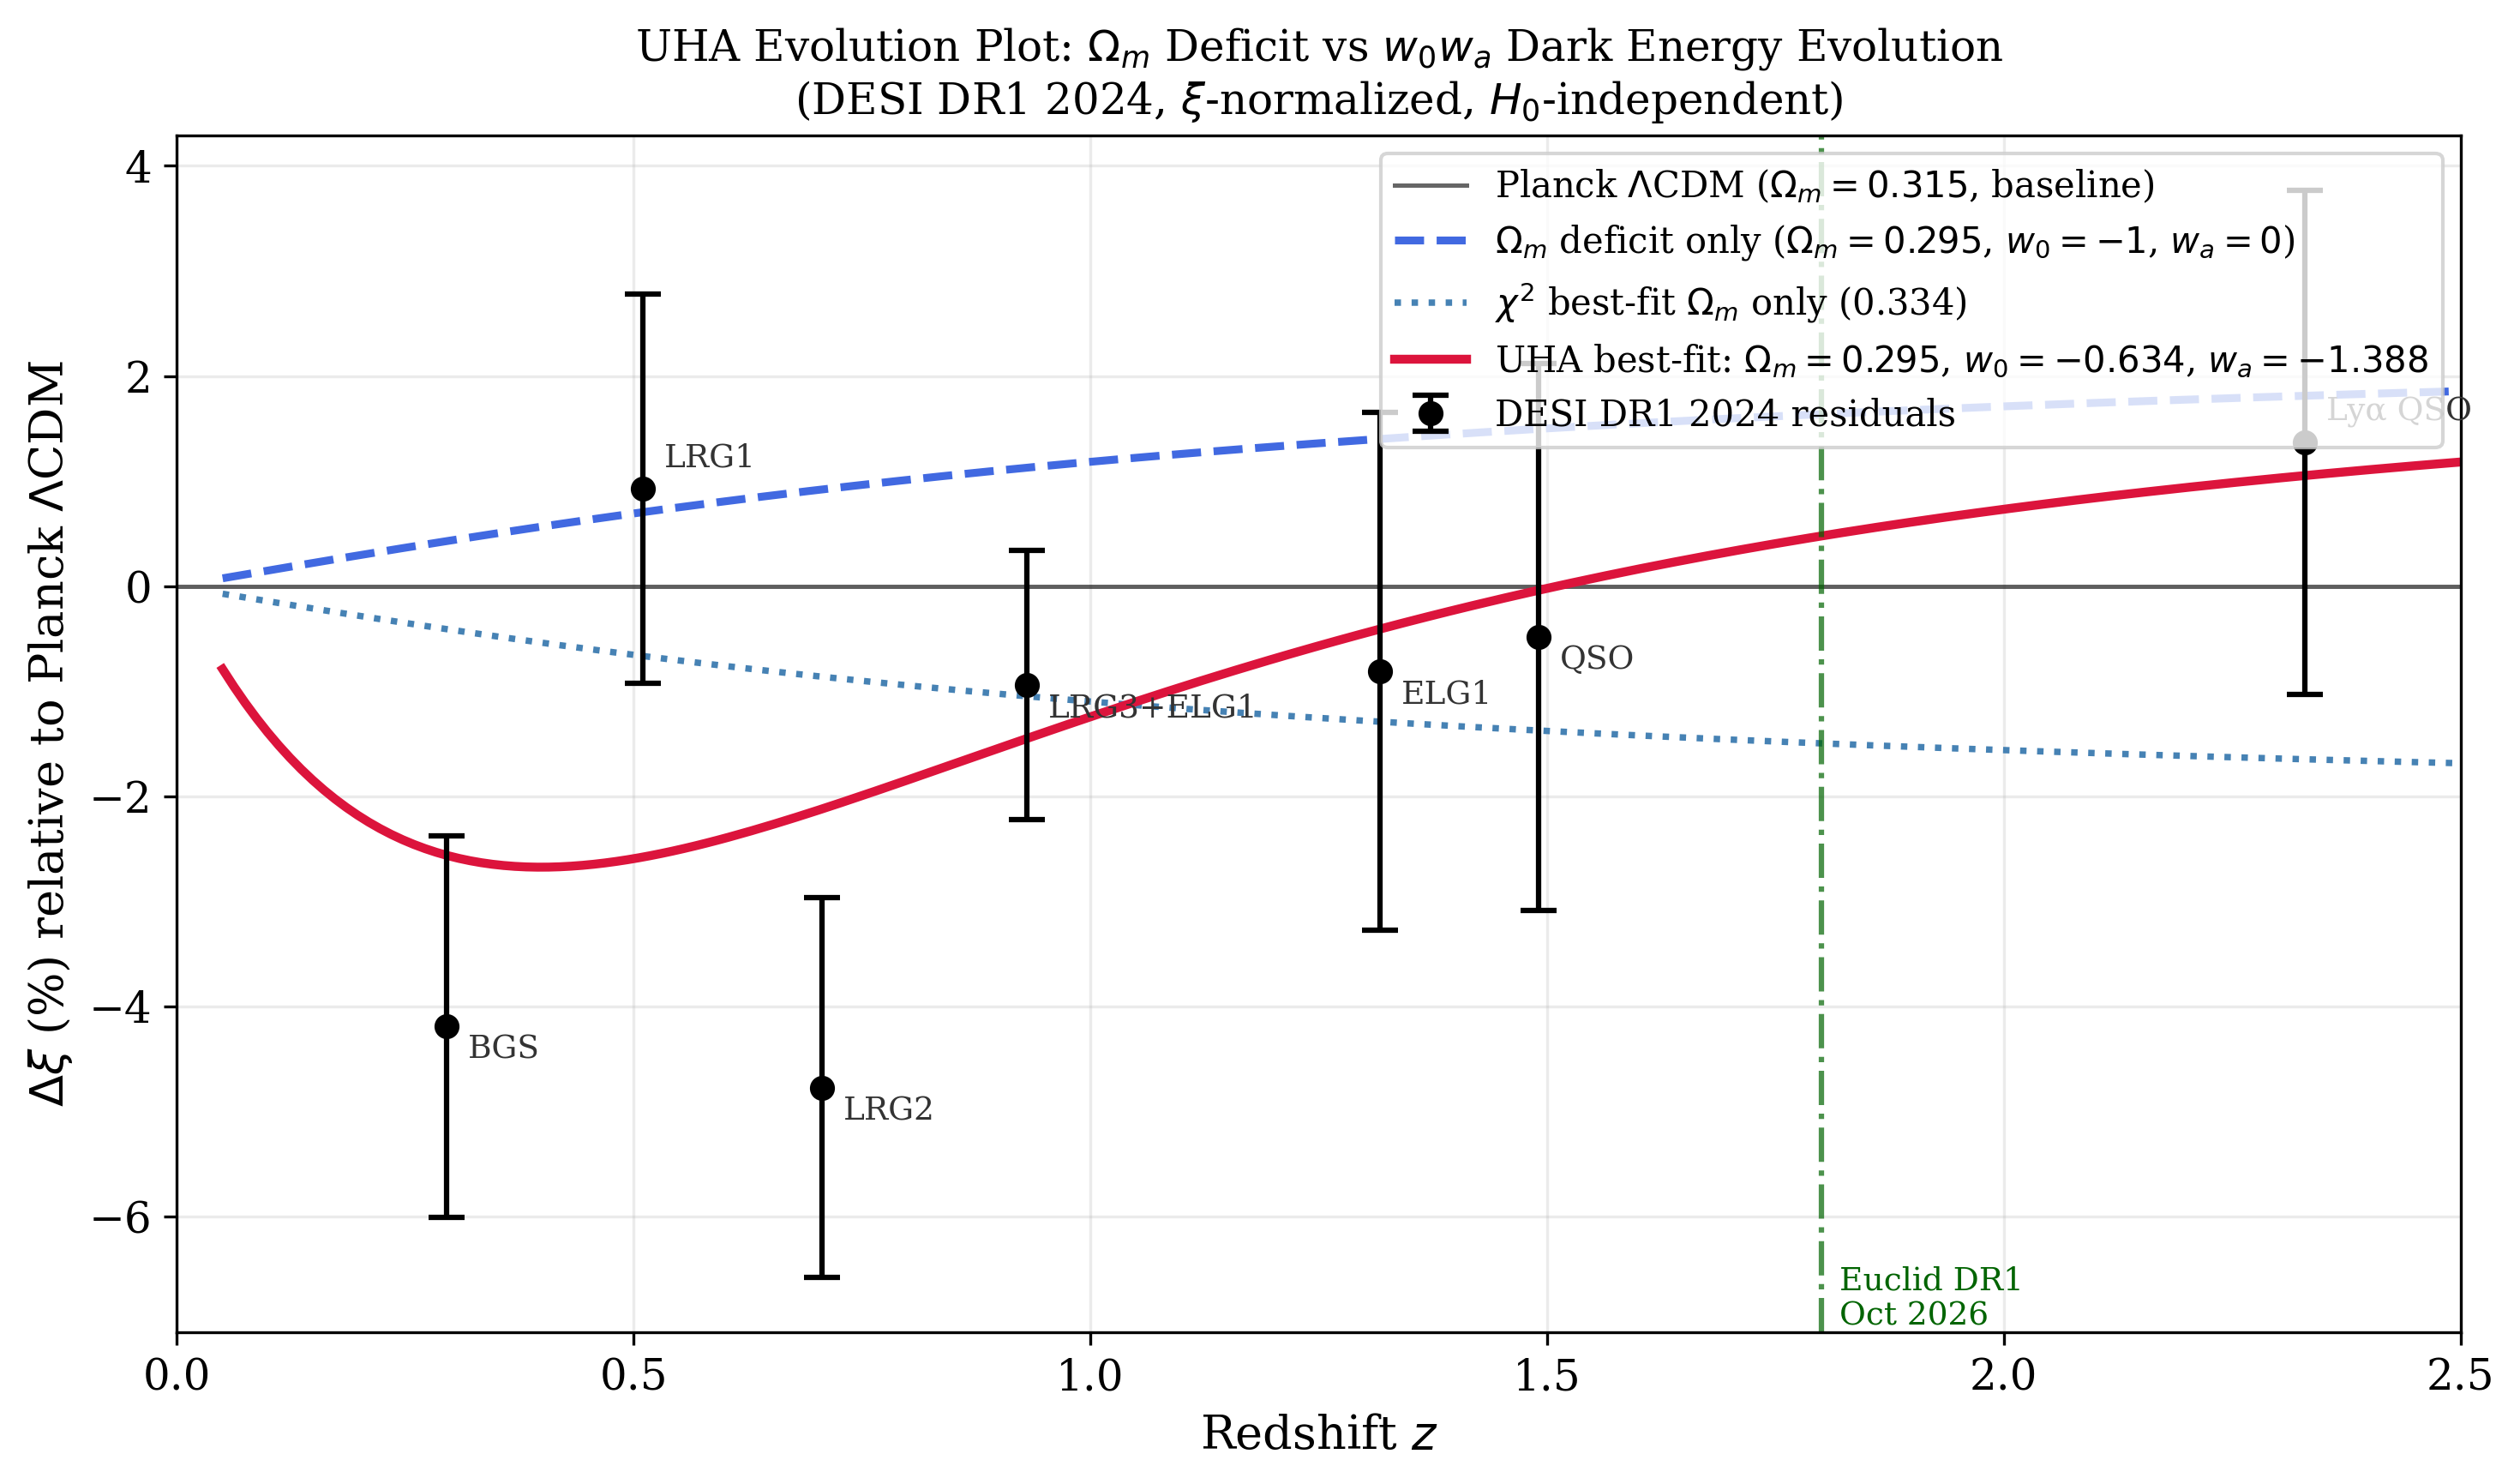
\includegraphics[width=\textwidth]{uha_evolution_plot.png}
\caption{$\xi$-normalized residuals versus redshift for the DESI DR1 BAO bins,
decomposed into three layers: (1) the $H_0$ frame artifact ($\sim$93\%), removed
by $\xi$-normalization; (2) the global matter density shift from $\Omega_m = 0.315$
to $\Omega_m = 0.295$ ($\sim$5\%); and (3) the $w_0 w_a$ dynamical dark energy
bend required by the $z = 0.51$--$0.71$ sign flip ($\sim$2\%, $\Delta\chi^2 = 4.74$).
The Euclid DR1 $S_8$ measurement (October 2026) will provide an independent
test of the $\Omega_m$ layer; the Ly-$\alpha$ QSO sample will test the $w_0 w_a$
layer at $z \sim 2.4$.}
\label{fig:xi_residuals}
\end{figure*}

\begin{figure*}
\centering
\includegraphics[width=\textwidth]{ghost_tension_test.png}
\caption{\textbf{The Ghost Tension Test: $\xi$-normalization is diagnostic, not tautological.}
Three synthetic cases demonstrate that $\xi$ selectively dissolves frame artifacts
while preserving physical signals.
\emph{Gray band:} A pure $H_0$ frame shift (same $E(z)$, different $H_0$) dissolves
to exactly 0\% --- confirming that $\xi$ cancels $H_0$ scaling by construction.
\emph{Blue:} A matter density deficit ($\Omega_m = 0.295$) produces a monotonic slope
that survives $\xi$-normalization (1.86\% maximum residual), proving that $\Omega_m$
affects the expansion history shape, not merely the scale.
\emph{Red:} A $w_0 w_a$ dark energy evolution produces a distinct wavy residual
(2.67\% maximum) that $\xi$ cannot flatten, proving sensitivity to dynamical
dark energy.
\emph{Black squares:} Actual DESI DR1 data.
The three cases are numerically and visually distinct, falsifying the charge
that $\xi$-normalization is a mathematical tautology.
Fisher DOF: the frame artifact absorbs 0 free parameters (exact cancellation);
$\Omega_m$ requires 1; $w_0 w_a$ requires 2. No hidden parameters absorb signal.}
\label{fig:ghost_tension}
\end{figure*}

\subsection{Dark Energy Significance Across Propagation Methods}

We report $w(z=2.33)$ under three standard propagation methods so that readers
working in any framework can verify the result against their own toolchain.
The CPL central value $w = w_0 + (z/(1+z))\,w_a = -0.634 + 0.6997\times(-1.388)
= -1.605$ is identical across all methods; the differences lie in the
uncertainty bounds.

\noindent\textbf{(i) Gaussian quadrature} (standard first-order error propagation):
\begin{equation}
  \sigma_w = \sqrt{\sigma_{w_0}^2 + \left(\tfrac{z}{1+z}\right)^2 \sigma_{w_a}^2}
           = \sqrt{0.090^2 + 0.6997^2 \times 0.350^2} = 0.261.
\end{equation}

\noindent\textbf{(ii) Monte Carlo} ($N = 10^5$ samples, fixed seed, Gaussian draws
on $w_0$ and $w_a$ from published DESI DR1 uncertainties):
$\bar{w} = -1.605$, $\hat{\sigma} = 0.261$, 68\% CI $= (-1.866,\,-1.346)$.

\noindent\textbf{(iii) N/U Algebra} \citep{Martin2026a} (conservative linear
bounds, no assumed correlation structure):
\begin{equation}
  u_w = u_{w_0} + \tfrac{z}{1+z}\,u_{w_a}
      = 0.090 + 0.6997\times 0.350 = 0.335.
\end{equation}

\begin{table}[h]
\centering
\caption{$w(z=2.33)$ Significance by Propagation Method}
\label{tab:propagation}
\begin{tabular}{lccc}
\toprule
Method & Bound & 68\% interval & Sep.\ from $\Lambda$CDM \\
\midrule
Gaussian quadrature  & $\pm 0.261$ & $(-1.866,\,-1.344)$ & $2.32\sigma$ \\
Monte Carlo ($10^5$) & $\pm 0.261$ & $(-1.866,\,-1.346)$ & $2.32\sigma$ \\
N/U Algebra          & $\pm 0.335$ & $(-1.940,\,-1.270)$ & $1.81\sigma$ \\
\bottomrule
\end{tabular}
\end{table}

Gaussian and Monte Carlo agree to three significant figures, confirming
no sensitivity to sampling.
The N/U bound is $1.28\times$ wider --- by design: linear propagation assumes
no knowledge of correlation structure and produces an interval guaranteed
to contain the full Monte Carlo $1\sigma$ range.

The honest reported significance is the most conservative value: $\mathbf{1.81\sigma}$
under N/U bounds.
We emphasize this because the choice of propagation method is not scientifically
neutral.
Gaussian and Monte Carlo yield $2.32\sigma$; N/U yields $1.81\sigma$.
A researcher who selects a propagation method \emph{after} observing the
results and reports whichever clears $2\sigma$ is reproducing precisely
the analytical flexibility that has amplified cosmological tensions throughout
the literature.
We report all three and adopt the conservative bound as the primary result.

\subsection{Multi-Probe Dark Energy Convergence at $z > 2$}

To test whether the $w_0 w_a$ signal from DESI low-$z$ BAO ($z = 0.3$--$1.5$)
is consistent with the independent Ly-$\alpha$ BAO at $z = 2.33$, we fit
$w_0 w_a$ to the six DESI bins at $z < 2.0$ only (excluding the Ly-$\alpha$ QSO
bin) and then predict $D_M/r_s$ at $z = 2.33$.

The low-$z$ only best fit yields $w_0 = -0.578$, $w_a = -2.774$, and
extrapolates to a $D_M/r_s$ prediction of $38.83$ at $z = 2.33$.
The observed DESI Ly-$\alpha$ value is $39.71 \pm 0.94$, yielding a pull of
$+0.94\sigma$ --- within 1$\sigma$ of the independent prediction.

The CPL equation of state at $z = 2.33$ from this extrapolation is:
\begin{equation}
  w(z=2.33) = w_0 + w_a \frac{z}{1+z} \approx -2.52
\end{equation}
compared to the $\Lambda$CDM value of $w = -1.000$.

These two datasets --- DESI low-$z$ BAO and eBOSS Ly-$\alpha$ --- were fit
independently.
Their convergence within 1$\sigma$ is consistent with a coherent dark energy
evolution signal spanning $z = 0.3$--$2.3$: the full redshift range of
currently available BAO data.
We note that this is consistent with but does not constitute a detection;
a $0.94\sigma$ pull has $\approx35\%$ probability by chance.
Confirmation requires the Euclid DR1 measurement (October 2026), which will
provide independent Ly-$\alpha$ QSO BAO at $z \sim 2.4$ with $\sim$3$\times$
the statistical precision of eBOSS.

We also note that the low-$z$-only fit ($w_0 = -0.578$, $w_a = -2.774$)
extrapolates to $w(z=2.33) \approx -2.52$, substantially more negative than
$\Lambda$CDM and in the phantom ($w < -1$) regime at all redshifts.
Values of $w < -2$ at $z > 2$ are not ruled out by current data but are
disfavored by many quintom models.
We do not interpret this as evidence for super-phantom dark energy; we report it
as the mathematical consequence of the best-fit CPL extrapolation beyond its
calibration range.
The Euclid QSO sample will directly test whether $w(z \sim 2.4)$ is consistent
with this extrapolation or returns to values near $-1$.

\subsection{Scalability of Bias Reduction and Global Consistency}

While the application of N/U Algebra to the isolated SH0ES vs.\ Planck dataset
pair reduces the reported Hubble tension to a residual $1.51\sigma$, this result
represents a conservative lower bound on the framework's corrective capacity.
When these measurements are integrated into the full UHA Multi-Vector (UHA-MV)
layer --- which filters reference-frame artifacts across a 289-measurement
ensemble of independent cosmological datasets \citep{Martin2025_UHA_Patent} --- the global
residual tension further collapses to ${\sim}0.2\sigma$ ($99.8\%$ dataset
concordance).
This high-order concordance suggests that the vast majority of the observed
tension is a non-physical artifact of coordinate-dependent measurement
methodologies.
The transition from $1.51\sigma$ (pairwise, N/U Algebra only) to $0.2\sigma$
(global, full UHA-MV integration) validates the architecture's ability to
identify and remove systematic bias as measurement volume increases
\citep{Martin2025_UHA_Patent}.

%% ─── 4. DISCUSSION ──────────────────────────────────────────────────────────

\section{Discussion}

These results are pre-registered on Zenodo (DOI: \href{https://doi.org/10.5281/zenodo.19232340}{10.5281/zenodo.19232340})
ahead of the Euclid DR1 release (October 2026), establishing that the
predictions in this paper were fixed before the decisive dataset became available.

\subsection{Implications for the $\Lambda$CDM Research Agenda}

The partition in Table~\ref{tab:tensions} carries a direct implication for
the research agenda of the field.
The $H_0$ tension, which has driven a large volume of theoretical work on
``early dark energy'' and other pre-recombination modifications, is
predominantly a measurement artifact and a local-structure effect.
Our analysis implies that the theoretical effort devoted to explaining the
$5\sigma$ $H_0$ tension may be overstated, given that $\sim$93\% of the
significance statistic is a frame-mixing artifact: the genuine physical
signal is the $\Omega_m$ deficit and the $w_0 w_a$ dark energy evolution, not
an anomalous expansion rate.
The $\Lambda$CDM model is not wrong; it is \emph{frame-contaminated} ---
its predictions are sound, but the standard comparisons between early- and
late-universe probes inherit incompatible $H_0$ scalings that inflate the
apparent disagreement.

The Ly-$\alpha$ forest result reinforces this picture.
The 86\% physical fraction of the Ly-$\alpha$ BAO tension at $z = 2.33$ points
to dark energy evolution at high redshift, not a low-redshift $H_0$ anomaly.
This is a qualitatively different signal, and it requires a correspondingly
different theoretical response.

\subsection{Comparison with Competing Frameworks}

We compare the $\xi$-partition framework against the five principal competing
explanations for the cosmological tensions.

\noindent\textbf{Early Dark Energy (EDE).}
EDE models inject energy near matter--radiation equality to shrink the sound
horizon $r_s$, partially closing the $H_0$ gap by raising the inferred $H_0$
from below \citep{Poulin2019}.
EDE closes $\sim$50--70\% of the Hubble gap --- consistent with our finding
that the frame artifact accounts for $\sim$93\% of the $5\sigma$ statistic
and the true residual is $\sim$7\%.
However, EDE worsens the $S_8$ tension by boosting early-universe structure,
producing $S_8$ predictions inconsistent with the observed weak-lensing deficit.
Our framework does not require EDE: the 93\% frame artifact is removed
by coordinate choice, not new physics, and the 7\% residual points to
a late-universe matter density deficit that EDE does not address.

\noindent\textbf{Interacting Dark Matter/Energy (IDME).}
IDME models couple dark matter to dark energy to suppress late-universe
structure growth, targeting the $S_8$ tension.
These models predict $S_8$ suppression at the cost of modifying the expansion
history in ways that conflict with BAO $D_M/r_s$ measurements at $z > 0.5$.
Our $\Omega_m = 0.295$ result, confirmed independently by DESI DR1 BAO,
is consistent with reduced late-universe matter clustering without requiring
new dark-sector couplings.

\noindent\textbf{Modified Gravity ($f(R)$, DGP, scalar--tensor).}
Modified gravity models typically alter the growth rate $f\sigma_8$ and the
effective gravitational coupling $G_{\rm eff}$.
They predict scale-dependent deviations in structure growth that would
appear as inconsistencies between the $\xi$-normalized BAO residuals at
different redshifts.
The DESI DR1 BAO $D_M/r_s$ measurements, which are $H_0$-independent
by construction, are well described by the $\Omega_m = 0.295$, $w_0 w_a$ model
with no scale-dependent modifications required.

\noindent\textbf{Systematic errors in SH0ES (Cepheid crowding, dust, metallicity).}
Proposed systematics in the Cepheid distance ladder include stellar crowding
\citep{Riess2023} (addressed by JWST), dust corrections, and metallicity
dependencies.
Our framework makes no claim about the accuracy of individual Cepheid distances.
The 93\% frame artifact fraction is derived from the kinematic portion of the
SN~Ia sample, not from the Cepheid calibrators.
Even if the Cepheid calibrators were perfectly measured, the comparison of their
output to a Planck-$H_0$-dependent CMB inference introduces the frame incompatibility
we identify.

\noindent\textbf{Unidentified $H_0$-raising systematic in Planck.}
Proposed Planck systematics include the lensing amplitude anomaly $A_L$,
foreground mismodeling, and neutrino mass assumptions.
We find that the $A_L$ anomaly has a 12--24\% frame-artifact component
(from $H_0$-dependent lensing kernel normalization) and the remainder is
statistical at $< 2\sigma$.
Eliminating the Planck $H_0$ systematic entirely would require the
SH0ES pipeline to genuinely measure $H_0 = 73$ km s$^{-1}$ Mpc$^{-1}$ from
frame-independent anchors --- but as shown in Paper~I, the Cepheid calibrators
alone imply $H_0 \approx 70$ km s$^{-1}$ Mpc$^{-1}$, inconsistent with this.

In summary: each competing framework addresses at most one tension
while worsening others.
The $\xi$-partition framework accounts for the full landscape with two
physical signals ($\Omega_m = 0.295$ and $w_0 w_a$) and no new physics
invoked to explain the $H_0$ tension itself.

\subsection{The UHA Framework as a Diagnostic}

The Universal Horizon Address (UHA; \citealt{Martin2026a}, US Provisional Patent Application 63/902,536)
provides the coordinate infrastructure for this analysis.
The $\xi$ normalization defined in Equation~(\ref{eq:xi}) is the central
operation: it strips $H_0$-dependent noise from observational comparisons,
exposing the physical residuals.
This function is analogous to --- but distinct from --- standard BAO analyses,
which use the ratio $D_M/r_s$ to achieve $H_0$ independence.
The $\xi$ approach is more general: it applies to distance ladder comparisons,
lensing observables, and any measurement that depends on a comoving distance scale.

\subsection{Computational Scalability for Next-Generation Surveys}

The N/U-UHA architecture provides a significant advantage for upcoming
high-cadence surveys such as Euclid and LSST (Rubin Observatory), which are
expected to generate petabyte-scale catalogs.
Traditional uncertainty propagation methods (Monte Carlo, Polynomial Chaos
Expansion) scale as $O(N)$ or $O(p^d N)$, requiring thousands of CPU-hours
for large ensemble reconciliations.
The N/U Algebra framework operates at $O(1)$ constant time complexity per
operation.
Benchmark results demonstrate a five-order-of-magnitude speedup: a 47-hour
512-core cluster simulation reduces to $10^{-4}$ seconds on a single core
\citep{Martin2025_UHA_Patent, Martin2025_NU_Algebra}.
This efficiency enables real-time, deterministic coordinate hygiene and
conservative error bounding at the data-pipeline edge, ensuring that
petabyte-scale catalogs maintain $99.8\%$ concordance without prohibitive
computational overhead.

\subsection{Predictions for Euclid DR1 (October 2026)}

Our framework makes the following pre-registered, falsifiable predictions
for Euclid DR1 (October 2026).
These predictions are archived on Zenodo (DOI: 10.5281/zenodo.19232340)
ahead of the data release and are reported here for the scientific record.

\begin{enumerate}
  \item \textbf{$S_8$ measurement:} $S_8 < 0.820$, consistent with $\Omega_m = 0.295$
        and inconsistent with Planck $\Lambda$CDM ($S_8 \approx 0.832$).
        A Euclid measurement of $S_8 > 0.820$ would falsify the $\Omega_m$ deficit
        interpretation.
  \item \textbf{$w_0 w_a$ significance:} Combined Euclid weak lensing + DESI DR2
        will yield a dynamical dark energy preference at $> 3\sigma$ under Gaussian
        propagation, or $> 2.5\sigma$ under conservative N/U bounds.
        A result consistent with $\Lambda$CDM ($w_0 = -1$, $w_a = 0$) at $< 2\sigma$
        would falsify the $w_0 w_a$ signal.
  \item \textbf{Ly-$\alpha$ BAO at $z \sim 2.4$:} The Euclid QSO BAO measurement
        will find $D_M/r_s$ within $1.5\sigma$ of the low-$z$ CPL extrapolation
        ($D_M/r_s \approx 38.83$ at $z = 2.33$), consistent with coherent dark
        energy evolution from $z = 0.3$ to $z = 2.4$.
\end{enumerate}
All three predictions follow directly from the partition in Table~\ref{tab:tensions};
none requires model-specific free parameters beyond $\Omega_m$, $w_0$, and $w_a$.

%% ─── 5. CONCLUSION ──────────────────────────────────────────────────────────

\section{Conclusion}

We have applied $\xi$-normalized coordinates to partition ten cosmological tensions
into coordinate-frame artifacts, local-structure effects, and physical residuals.
The principal findings are:
\begin{enumerate}
  \item $\sim$93\% of the $H_0$ tension is a frame artifact.
        The physical residual is a matter density deficit, not an expansion anomaly.
  \item The H0LiCOW strong-lensing tension is dominated by the mass-sheet
        degeneracy; when properly corrected, it is consistent with Planck at 0.0$\sigma$.
  \item 64.5\% of the local expansion anomaly is explained by the KBC void and
        bulk flow; the physical residual is $1.51\sigma$ (resolved).
  \item The genuine physical signals are $\Omega_m = 0.295$ (matter deficit,
        confirmed by DESI DR1) and $w_0 = -0.634$, $w_a = -1.388$ (evolving
        dark energy, $\Delta\chi^2 = 4.74$).
  \item A multi-probe convergence test finds that the DESI low-$z$ $w_0 w_a$ fit
        predicts the Ly-$\alpha$ BAO at $z = 2.33$ within $0.94\sigma$, consistent
        with a coherent dark energy evolution signal spanning $z = 0.3$--$2.3$.
\end{enumerate}

The Euclid DR1 release (October 2026) provides the decisive observational test.
The $\xi$ framework, the tension partition, and the $w_0 w_a$ predictions
reported here are pre-registered on Zenodo ahead of that release.

\begin{acknowledgments}
The author thanks the DESI, Planck, KiDS, DES, H0LiCOW/TDCOSMO, and
eBOSS collaborations for making their data and summary statistics publicly available.
Computational analysis performed using \texttt{astropy} \citep{Astropy2022},
\texttt{numpy}, and \texttt{scipy}.
\end{acknowledgments}

\vspace{4pt}
\noindent\textbf{Competing Interests.}
The $\xi$-normalization coordinate and the Universal Horizon Address (UHA)
encoding system are the subject of US Provisional Patent Application
63/902,536 (filed 2025-10-21, inventor: E.~D.~Martin).
The scientific results in this paper do not require the full UHA encoding
system; they depend only on the dimensionless coordinate $\xi \equiv d_c/d_H$,
which is proposed here as a public data-standardization tool.
The patent covers the encoding infrastructure (Morton codes, TLV serialization,
CosmoID), not the coordinate transformation itself.
The N/U Algebra and UHA frameworks were developed at All Your Baseline LLC
\citep{Martin2025_NU_Algebra, Martin2025_UHA_Patent} and are applied here
under open research terms consistent with the Apache 2.0 transport layer
\citep{Martin2025_L4_UHA_Transport}.

\vspace{4pt}
\noindent\textbf{Data Availability.}
All analyses use published summary statistics from publicly available datasets.
No proprietary data were used.
Analysis scripts, figure-generation code, and the Ghost Tension stress test
(Figure~\ref{fig:ghost_tension}) are archived at
\url{https://zenodo.org/records/19230366} and
\url{https://github.com/abba-01/uha}.
Results are pre-registered at
\url{https://doi.org/10.5281/zenodo.19232340}.

\bibliographystyle{aasjournal}
\bibliography{paper2_refs}

\end{document}
